\setAuthor{Jaan Kalda}
\setRound{lõppvoor}
\setYear{2006}
\setNumber{G 10}
\setDifficulty{10}
\setTopic{Dünaamika}

\prob{Kuulid}
\begin{wrapfigure}[8]{r}{0.3\textwidth}
	\begin{center}
		\vspace{-25pt}
		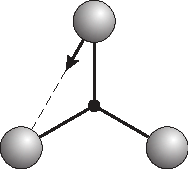
\includegraphics[width=\linewidth]{2006-v3g-10-yl}
	\end{center}
\end{wrapfigure}
Joonisel kujutatud süsteem koosneb kolmest võrdkülgse kolmnurga tippudes paiknevast kuulist massiga $m$ ja kolmest kergest vardast pikkusega $l$, mis on omavahel šarniirselt ühendatud (liigendiga). Süsteem lebab hõõrdevabalt siledal horisontaalpinnal. Ühte kuuli lükatakse teatud lühiajalise jõuga nii, et see omandab kiiruse $v_0$, mis on suunatud naaberkuuli poole. Leidke teiste kuulide kiiruste suunad ja moodulid ning kõigi kuulide kiirendused vahetult peale esimese kuuli lükkamist.

\hint
Teisest ja kolmandast kuulist koosnevale süsteemile mõjus esimese kuuli lükkamise ajal esimese varda sihiline jõud, sest teatavasti mõjuvad kergetele varrastele vaid varda sihilised pinged. Lisaks peab esimese kuuli lükkamise ajal kehtima varraste venimatuse tingimus.

Kiirenduse leidmiseks on süsteemi mugav vaadelda šarniirse ühenduspunktiga kaasa liikuvas ja kiirenevas taustsüsteemis ning seejärel rakendada Newtoni II seadust.

\solu
Teisest ja kolmandast kuulist koosnevale süsteemile mõjus sel ajal, kui esimest kuuli lükati, esimese varda sihiline jõud, sest teatavasti mõjuvad kergetele varrastele vaid varda sihilised pinged. Seega nihkus šarniirne ühenduspunkt esimese varda sihiliselt ning teine ja kolmas kuul omandasid sümmeetria tõttu ühesugused kiirused. Šarniirse ühenduspunkti kiirus on $v_s = v_0 \cos \ang{30}$, sest esimese varda pikkus ei muutu. Et nii teisele kui kolmandale kuulile mõjub ainult varda sihiline jõud, siis nende kiirus on ka varda sihiline; varda venimatusest juhtivalt $v_2 = v_3 = v_s \cos \ang{60} = v_0 \sqrt 3/4$.

Pinged varrastes on võrdsed, sest šarniirse ühenduspunkti massi võime lugeda nulliks ning talle mõjuv resultantjõud peab olema 0 ja jõudude tasakaalust tuginevalt peab varraste pingetest moodustuma võrdkülgne kolmnurk. Olgu varraste pinge $T$. Seega on kõigi kuulikeste kiirendused võrdsed, $a_k = T /m$. Läheme šarniirse ühenduspunktiga seotud kulgevalt liikuvasse taustsüsteemi, mis liigub kiirendusega $\vec a$. Selles süsteemis on esimese kuuli kiirus $u_1 = v_0/2$ ning teiste kiirus $u_2 = v_s \sin \ang{60} = \frac{3}{4} v_0$. Selles süsteemis liiguvad kuulid ringjoont mööda. Iga kuuli jaoks saame välja kirjutada jõudude tasakaalu tingimuse projekteerituna vastava varda sihile (siis kaob vajadus teada kuulikese ringliikumise tangetsiaalkiirendust, sest see on teljega risti). Teise ja kolmanda kuuli tasakaalutingimusi võrreldes selgub, et inetrsijõu $-m\vec a$ projektsioon kummalegi teljele peab olema üks ja sama, st $\vec a$ peab olema esimese varda sihiline. Seega saame kaks võrrandit:
\[
\begin{aligned}
mu_1^2/l + a &= T,\\
mu_2^2/l - a/2 &= T.
\end{aligned}
\]
Elimineerides neist võrrandeist $a$, saame
\[
T=\frac{1}{3} \frac{m}{l}\left(u_{1}^{2}+2 u_2^{2}\right)
\]
ning otsitava kiirenduse
\[
a_{k}=T / m=\left(u_{1}^{2}+2 u_2^{2}\right) 3 l=\frac{11}{24} v_{0}^{2} / l.
\]
\probend